\section{Methodology} % (fold)
\label{sec:methodology}
 
\subsection{LDA Model} % (fold)
\label{sub:lda_model}

Constructing the topic variables requires two components: First is a probability that each product belongs to each specific topic. Second is a measurement for each consumer that links a consumer's personal purchase profile with each topic. Constructing the first proves to be quite simple; the topic modeling library \cite{lda} from CRAN's library of packages is used for the purposes of this paper\footnote{It's similar to the topic modeling packages like Scikit Learn for Python.}. The model requires a document-term matrix to return the beta and gamma coefficients. The topic modeling library provides useful functions to tokenize and remove any stop-words from the documents. by casting the documents, one obtains the document terms matrices required for the model\footnote{Figure 14 in the Appendix shows the word-count per product description, after all the documents are tokenized and the stop words removed}. The beta coefficients, or the word-topic probabilities, represents the probabilities for each word belonging to each topic. The gamma coefficients, or the document-topic probabilities, represent the probabilities of a document belonging to each of the topics. The gamma matrix is used for the purpose of this paper. Each product's description thus has a probability of belonging to a topic. However, this does not yield a particular distribution for each consumer. To get a distribution for each consumer over the topics, one needs to consider the link between the gamma matrix and a measurement for household "interest" in a product. 

\

A simple way to to connect the gamma matrix with each individual is to have a normalized unit root value per topic per consumer. To do this, I counted the number of times a consumer bought a particular product. However, the surveys were conducted randomly and thus some households repeated in the sample. To account for this, I averaged the amount of times of those households purchased products over the amount of times they repeated in the sample. This resulted in the following consumer product propensity matrix:

\begin{equation}\centering
	CPP = \left[ {\begin{array}{*{20}{c}}
{NEWID}&{product}&n\\
{1292531}&{10120}&{1.0}\\
\begin{array}{l}
1292531\\
 \vdots 
\end{array}&\begin{array}{l}
200110\\
 \vdots 
\end{array}&\begin{array}{l}
1.5\\
 \vdots 
\end{array}
\end{array}} \right]
\end{equation}


 
 Where \textit{NEWID} is a vector of the consumers, \textit{product} is the UCC code for each product and \textit{n} the average amount of times a consumer purchased a product\footnote{Figure 15 in the Appendix shows a visual representation of the CPP matrix, where households are on the y axis and products on the x axis; it simply shows that some products are frequently purchased.}. Thereafter, I then multiplied the amount of times, n, each product was purchased by each consumer by the probability (gamma value for that product) that the product belonged to a certain topic. Thereafter I took the unit root of each topic with respect to each topic and particular household to normalize the value:




\begin{equation}\centering
	Topi{c_i}(k) = \frac{{\sum\limits_{j = 1}^{509} {({\gamma _j}(k)*{n_{ij}})} }}{{\sqrt {\sum\limits_{k = 1}^K {{{\left( {\sum\limits_{j = 1}^{548} {({\gamma _j}(k)*{n_{ij}})} } \right)}^2}} } }}
\end{equation}



where \textit{i} is each individual household, \textit{j} is each individual product and \textit{k} is each individual topic. The \textit{n} represents the average amount of times a consumer purchased a particular product. Figures 1 and 2 visually represent this process. 
\


\begin{figure}[!h]
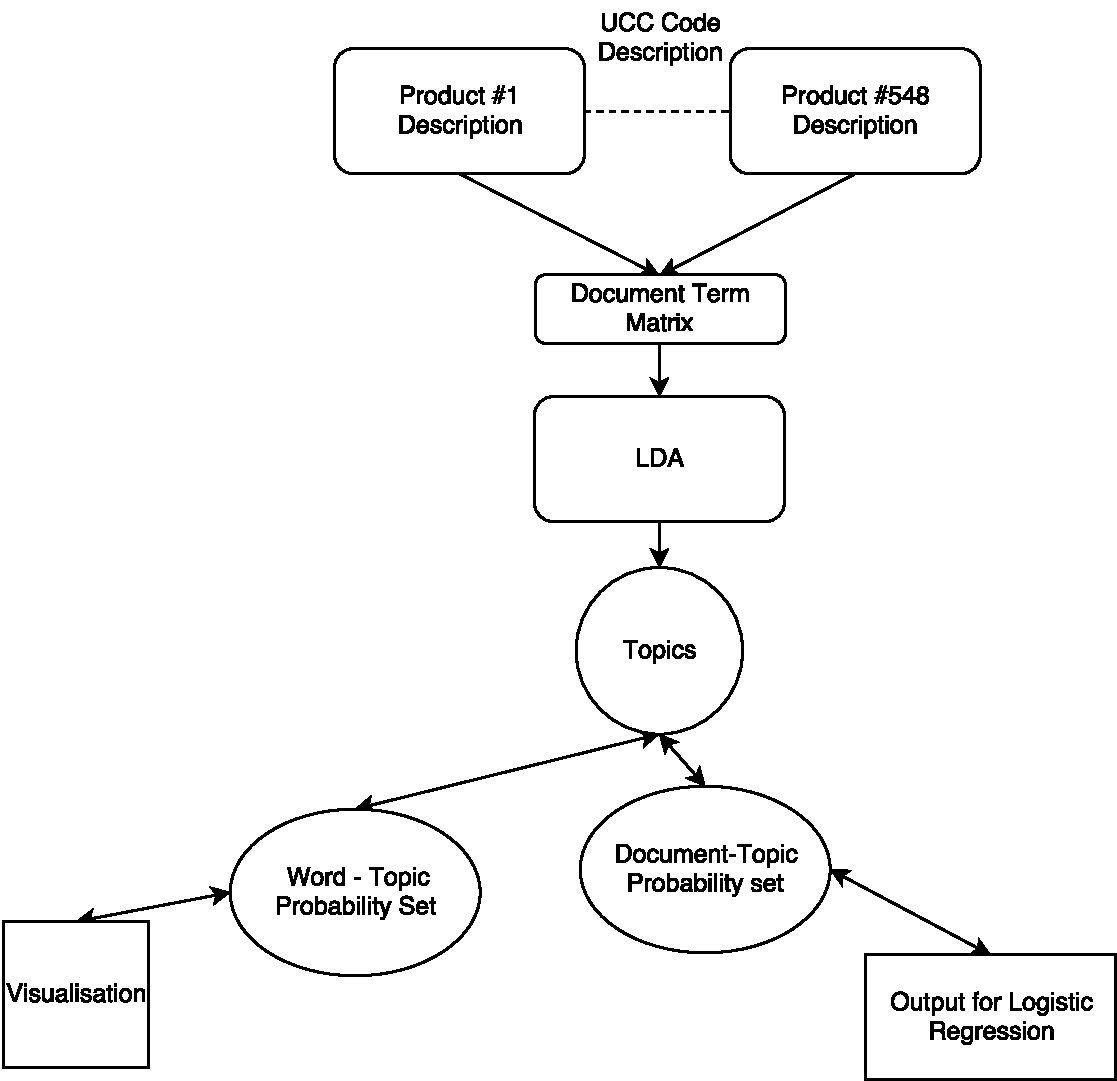
\includegraphics[width=1\textwidth]{/Users/charlvanschoor/Documents/Gottingen/ML/ML-Applications-CVS/LDA_consumer_analysis/paper/content/graphs/LDA.pdf}
\caption{LDA Input-Output Layout}
\end{figure}

\begin{figure}[!h]
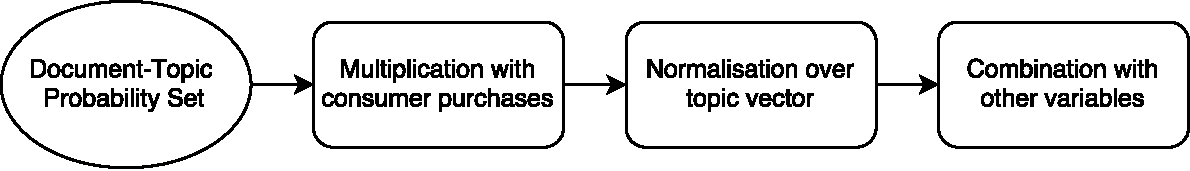
\includegraphics[width=1\textwidth]{/Users/charlvanschoor/Documents/Gottingen/ML/ML-Applications-CVS/LDA_consumer_analysis/paper/content/graphs/norm.pdf}
\caption{Topics to Final Dataset Layout}
\end{figure}

% subsection lda_model (end)

\subsection{Logistic regression} % (fold)
\label{sub:logistic_regression}

The second goal of the paper is to identify which factors explain the most variation in gift purchasing behaviour. To do this I make use of a binomial logistic regression function which uses a logistic distribution log-likelihood function\footnote{The programming software R comes standard with Generalized Linear Models, of which the binomial GLM is used for this paper.}. The purpose of the logistic regression is to act as a baseline for predicting gift purchasing behaviour. The regression structure is as follows:

\

\begin{equation}\centering
GIF{T_i} = \sum\limits_{k = 1}^K {Topi{c_i}(k)}  + AG{E_i} + INCLAS{S_i} + EDUC{A_i} + STATE{_i} + SE{X_i}
\end{equation}
where $i = 1....N$ and $k = 1....L + K$

\

Each variable follows intuitively on the variables specified in the data section of this paper. Notice that the variable "Topic" is a summation over the topic vectors. The reason for this is that various amounts of topics are modeled for the purpose of this paper; the aim of which is to determine what set of topics is optimal for the highest prediction accuracy. The regressions thus models the log-likelihood, or intuitively the probability, that a consumer would purchase a gift or not. The decision boundary is set a 0.5, meaning that a probability below 0.5 is categorized as a 0, whereas a value equal to or above 0.5 is categorized as a 1. 


% subsection logistic_regression (end)

\subsection{Neural Network} % (fold)
\label{sub:neural_network}

The purpose of the neural network is to improve the prediction accuracy of the model, as this method is known to have a higher predictive capability than linear regression models. It has the ability to model non-linear relationships in a black box manner. This is however also the disadvantage of using this technique, as it does not allow for possible causal inference of the variables in the model. 

\

The neural network is set op to train and test the same model as that of the logistic regression model. The total dataset is constructed such that there are the same amount of households that have a value of 1 and 0 for GIFT. In other words, the training and testing datasets have reduced dimensions to account for possible pattern forming. If this is not done, the neural network learns to predict whether a household will not purchase a gift very well, but it falls short of predicting whether a household will purchase a gift. 

\

Moreover, the neural network is constructed with the Keras library that utilizes a TensorFlow backend. The model is set to have one hidden layer with 128 neurons as the nature of the dataset does not require the complexity of more hidden layers. The model includes a 30 percent dropout during training, as this helps the model from overfitting\citep{srivastava2014dropout}. The model also includes cross-validation during the training set to help detect over-fitting and to assist in hyper-parameter optimization. Furthermore, the hidden layer is fitted with a standard sigmoid activation function and the output layer is fitted with 
a softmax activation function\footnote{The decision for which activation function is made on intuition, as both activation functions yields better results.}. The model is fitted with adam as an optimization function, and a binary cross entropy loss function. Th model was set to run a smaller set of epochs with smaller bach sizes in order for it to train at a slower rate. Finally, the metrics used to validate the model is the accuracy of prediction in the test dataset and the optimization of the loss during training. 

% subsection neural_network (end)


% section methodology (end)
